\documentclass{amsart}

\usepackage[english]{babel}
\usepackage[utf8]{inputenc}
\usepackage{graphicx}
\usepackage{mathtools}
\usepackage{amsthm}
\usepackage{thmtools,thm-restate}
\usepackage{amsfonts}
\usepackage{hyperref}
\usepackage[singlelinecheck=false]{caption}
\usepackage[backend=biber,url=true,doi=true,eprint=false,style=alphabetic]{biblatex}
\usepackage{enumitem}
\usepackage[justification=centering]{caption}
\usepackage{indentfirst}
\usepackage{algorithm}
\usepackage{algpseudocode}
\usepackage{listings}
\usepackage[x11names, rgb]{xcolor}
\usepackage{tikz}
\usetikzlibrary{snakes,arrows,shapes}

\addbibresource{references.bib}

\makeatletter
\def\subsection{\@startsection{subsection}{3}%
  \z@{.5\linespacing\@plus.7\linespacing}{.1\linespacing}%
  {\normalfont\itshape}}
\makeatother

\makeatletter
\patchcmd{\@setauthors}{\MakeUppercase}{}{}{}
\makeatother

\DeclareMathOperator*{\argmin}{arg\,min}
\DeclareMathOperator*{\argmax}{arg\,max}
\DeclareMathOperator*{\Val}{\text{Val}}
\DeclareMathOperator*{\Ch}{\text{Ch}}
\DeclareMathOperator*{\Pa}{\text{Pa}}
\DeclareMathOperator*{\Sc}{\text{Sc}}
\newcommand{\ov}{\overline}

\newcommand\defeq{\mathrel{\overset{\makebox[0pt]{\mbox{\normalfont\tiny\sffamily def}}}{=}}}

\algrenewcommand\algorithmicrequire{\textbf{Input}}
\algrenewcommand\algorithmicensure{\textbf{Output}}

\captionsetup[table]{labelsep=space}

\theoremstyle{plain}

\newcounter{dummy-def}\numberwithin{dummy-def}{section}
\newtheorem{definition}[dummy-def]{Definition}
\newcounter{dummy-thm}\numberwithin{dummy-thm}{section}
\newtheorem{theorem}[dummy-thm]{Theorem}
\newcounter{dummy-prop}\numberwithin{dummy-prop}{section}
\newtheorem{proposition}[dummy-prop]{Proposition}
\newcounter{dummy-ex}\numberwithin{dummy-ex}{section}
\newtheorem{exercise}[dummy-ex]{Exercise}
\newcounter{dummy-eg}\numberwithin{dummy-eg}{section}
\newtheorem{example}[dummy-eg]{Example}

\numberwithin{equation}{section}

\newcommand{\set}[1]{\mathbf{#1}}
\newcommand{\pr}{\mathbb{P}}
\renewcommand{\implies}{\Rightarrow}

\newcommand{\bigo}{\mathcal{O}}

\setlength{\parskip}{1em}

\lstset{frameround=fttt,
	numbers=left,
	breaklines=true,
	keywordstyle=\bfseries,
	basicstyle=\ttfamily,
}

\newcommand{\code}[1]{\lstinline[mathescape=true]{#1}}
\newcommand{\mcode}[1]{\lstinline[mathescape]!#1!}


\title{%
  \noindent\rule{13cm}{1.0pt}\\
  \vspace{0.2cm}
  An Introduction to Sum-Product Networks
  \noindent\rule{13cm}{0.8pt}
}
\xdef\shorttitle{An Introduction to Sum-Product Networks}
\author[]{\normalsize\textbf{Renato Lui Geh}\\\small Computer Science\\Institute of Mathematics
  and Statistics\\University of São Paulo\\\texttt{renatolg@ime.usp.br}}

\begin{document}

\begin{abstract}
  Sum-Product Networks (SPNs) are deep probabilistic graphical models (PGMs) that compactly
  represent tractable probability distributions. Exact inference in SPNs is computed in time linear
  in the number of edges, an attractive feature that distinguishes SPNs from other PGMs. However,
  learning SPNs is a tough task. There have been many advances in learning both the structure and
  parameters of SPNs in the past few years. One interesting feature is the fact that we can make
  use of SPN's deep architecture and perform deep learning on these models. Since the number of
  hidden layers not only does not negatively impact the tractability of inference of SPNs but also
  augments the representability of this model, it is very much desirable to continue research on
  deep learning of SPNs. In this article we seek to produce a tutorial on Sum-Product Networks in
  a simpler, clearer way then how it is currently written in literature. We will introduce SPNs
  and explain how knowledge is represented in this model, how to perform exact inference and
  describe and analyse in detail a simple structural learning algorithm.
  \vspace*{-3.5em}
\end{abstract}

\maketitle

\section{Introduction}

Conventional probabilistic graphical models (PGMs) can compactly represent complex probability
distributions and perform sub-exponential time inference through approximate methods. They are able
to learn from data accurately and have very expressive semantics. However, exact inference in the
general case is intractable. The alternative to exact inference is through the use of approximation
algorithms. Unfortunately, approximate inference is at times unpredictable and analysis of these
algorithms is very difficult.

Sum-Product Networks (SPNs) are deep PGMs that are able to compactly represent tractable
probability distributions. Inference in SPNs is computed in time linear in the number of edges of
the graph, where the number of edges is at most polynomial in the number of variables of the
distribution. SPNs are represented by a DAG where internal nodes are either sum or product nodes.
Leaf nodes are univariate distributions, though recent work on SPNs have shown that multivariate
distributions are also allowed as leaves~\cite{id-spn}. Learning of SPNs can be achieved through
subsequent clusterings of both variables and instanciations, where sum nodes can be seen as
mixtures of distributions and product nodes as variable independencies. An interesting feature of
SPNs is its deep architecture. As shown in Delalleau and Bengio's work~\cite{shallow-vs-deep},
deep SPNs have more representative power than shallow SPNs. Poon and Domingos, on the innaugural
SPN article~\cite{poon-domingos}, were able to learn accurate deep SPNs with 36 layers, as opposed
to the few, less than ten layers that is typically learned in other deep models.

In this article we will provide a comprehensive description of Sum-Product Networks, from its graph
representation and how to perform exact polynomial time inference, to describing and analysing our
implementation of the structural learning algorithm introduced in~\cite{gens-domingos}, a learning
algorithm that is able to learn SPNs of potentially tens of layers.

\section{Sum-Product Networks}

A Sum-Product Network is a DAG where nodes can either be sums, products or leaves. In this section
we will present two definitions of SPNs. The first one can be considered ``low level'', whilst the
second carries heavier semantics due to properties we shall enumerate in this section. These
classifications of ``low level'' vs ``high level'' will become clearer as we progress through this
section.

\subsection{Network Polynomials}

Before we define SPNs more formally, we need to understand network polynomials. First introduced by
Darwiche~\cite{diff-approach-darwiche}, a network polynomial is a multilinear function over the
variables of an unnormalized distribution. Computing the marginals of the distribution through its
network polynomial is possible by setting all indicator variables to values consistent with
evidence. The partial derivatives of the network polynomial can be seen as conditioning the network
polynomial to a given event.

Network polynomials are not that attractive by themselves, as the number of terms in the polynomial
is exponential in the number of variables. Arithmetic circuits (ACs) are a way of representing
network polynomials with a polynomial number of terms. However, ACs are just another way of
compiling a Bayesian network into a polynomial-sized model for tractable distributions.

\begin{definition}[Network polynomial] Let $\mathcal{N}$ be a Bayesian network over set of
  variables $\mathbf{X}$. Let $Pa(X)$ be the set of parents of variable $X$. The network polynomial
  of $\mathcal{N}$ is given by
  \begin{equation*}
    f=\sum_{\mathbf{x}} \prod_{X, \Pa(X) \sim \mathbf{x}} \lambda_X \theta_{X|Pa(X)}
  \end{equation*}
  where $\mathbf{x}$ is the set of possible instantiations of $\mathbf{X}$ and $X \sim x$ means
  that $X$ is consistent with instantiation $x$.
\end{definition}

\begin{example}
  Let $\mathcal{N}=A\to B$ be a Bayesian network where $\mathbf{X}=\{A, B\}$ is the set of binary
  variables of $\mathcal{N}$. The network polynomial of $\mathcal{N}$ is given by the multilinear
  function
  \begin{equation*}
    f=\lambda_a\lambda_b\theta_{b|a}\theta_{a}+\lambda_a\lambda_{\ov{b}}\theta_{\ov{b}|a}\theta_a+
    \lambda_{\ov{a}}\lambda_b\theta_{b|\ov{a}}\theta_{\ov{a}}+\lambda_{\ov{a}}\lambda_{\ov{b}}
    \lambda_{\ov{b}|\ov{a}}\lambda_{\ov{a}}
  \end{equation*}
\end{example}

The indicator variables of a variable $X$ represent the possible configurations of $X$. Let
$\Val(X)$ be the set of possible values of variable $X$ and $m=|\Val(X)|$. Then the set of
indicator variables of $X$, denoted by $\boldsymbol{\lambda}_X$ has elements $\lambda_X^1,
\lambda_X^2,\ldots,\lambda_X^m$. A variable $X$ is consistent with instantiation $x$ if the
indicator variable that agrees with $x$ is set to $1$ and the other indicator variables of $X$ are
set to $0$. If there is no instantiation concerning variable $X$, then all indicator variables of
$X$ are set to $1$.

\begin{example}
  Let $\mathbf{X}=\{X_1,X_2,X_3,X_4\}$ be the set of binary variables of a network polynomial $f$.
  A variable $X_i$ can be evaluated as either $0$ or $1$. Let $\mathbf{e}=\{X_1=1,X_2=0,X_3=1\}$ be
  the evidence set. Computing the marginals of $f$ can be done by setting all indicator variables
  consistent with $\mathbf{e}$\\
  \begin{align*}
    &\lambda_{X_1}^0=0 &\hspace{35pt} \lambda_{X_1}^1=1\\
    &\lambda_{X_2}^0=1 & \lambda_{X_2}^1=0\\
    &\lambda_{X_3}^0=0 & \lambda_{X_3}^1=1\\
    &\lambda_{X_4}^0=1 & \lambda_{X_4}^1=1
  \end{align*}
\end{example}

The partial derivative of a network polynomial by a certain variable corresponds to conditioning
the polynomial to a certain event. By computing $\partial f/\partial \lambda_X(\mathbf{e})$, we are
merely setting the indicator variables consistently with $\mathbf{e}$. This leads to the theorem:

\begin{theorem} Let $\mathcal{N}$ be a Bayesian network representing probability distribution $\Pr$
  and having network polynomial $f$. For every variable $X$ and evidence $\mathbf{e}$, we have
  \begin{equation*}
    \frac{\partial f}{\partial \lambda_X}(\mathbf{e})=\Pr(x,\mathbf{e}\setminus\{X\})
  \end{equation*}
\end{theorem}

\subsection{Representing Sum-Product Networks}

Sum-Product Networks are closely related to network polynomials and arithmetic circuits. It can be
seen as a way of representing the network polynomial. Graphically, a Sum-Product Network is a DAG
with internal nodes as sums and products and leaves as indicator variables.

\begin{definition}
  An SPN $S$ is a DAG with two types of internal nodes: sums and products. A sum node is a node
  whose value is defined by $v_i=\sum_{j \in Ch(i)} w_{ij}v_j$, where $v_i$ is the value of sum
  node $i$, $\Ch(i)$ is the set of children of node $i$, $w_{ij}$ is the non-negative weight
  associated with directed edge $i\to j$ and $v_j$ is the value of node $j$. The value of a product
  node $i$ is given by $v_i=\prod_{j\in Ch(i)} v_j$. A leaf node is always an indicator variable.
  Its value is the value of the indicator variable. The value of $S$ is the value of the root node
  of $S$.
\end{definition}

An arbitrary node $i$ of an SPN $S$ is itself an SPN\@. We will denote the sub-SPN rooted at $i$ as
$S_i$. Although the weights of a sum node may take any non-negative value, if all the weights from
a sum node sum to one, then that node is normalized. If all sum nodes in the SPN are normalized,
then the SPN is normalized and its partition function will be $1$. Otherwise the partition function
is the value of $S$ when all indicator variables are set to $1$. Such function will be denoted as
$S(*)$. It was recently proven that normalized SPNs have as much representability power as
unnormalized SPNs~\cite{theoretical-spn}. The scope of an SPN is the set of variables that are
present in it. The same applies to each sub-SPN\@. A variable is in an SPN if any of its indicator
variables is a leaf in that SPN\@. We will denote the scope of an SPN $S$ as $\Sc(S)$. The elements
of $\Sc(S)$ are the variables present in $S$.

\begin{definition}[Validity]
  An SPN is valid if and only if it correctly computes the probability of evidence of the
  probability distribution it represents.
\end{definition}

\begin{definition}[Completeness]
  An SPN $S$ is complete if and only if, for every sum node $i$ in $S$, all children of $i$ have
  the same scope.
\end{definition}

\begin{definition}[Consistency]
  An SPN $S$ is consistent if and only if, for every product node $i$ in $S$, a variable present in
  $i$ has the same value as the same variable in the descendents of $i$.
\end{definition}

\begin{theorem}
  An SPN is valid if it is complete and consistent.
\end{theorem}

This theorem states that an SPN computes its value correctly if it is complete and consistent.
However, this does not exclude the possibility of correctly computing the probability of evidence
of incomplete and inconsistent SPNs.

\begin{definition}[Decomposability]
  An SPN $S$ is decomposable if and only if, for every product node $i$ in $S$, every pair of
  children of $i$ have disjoint scopes with each other.
\end{definition}

\begin{proposition}\label{decimpliescons}
  Decomposability implies in consistency.
\end{proposition}

\begin{proof}
  It is easy to see that decomposability implies in consistency. For each product node $i$ in $S$,
  let $u$ and $v$ be a pair of children of $i$. If $S$ is decomposable, then $\Sc(u)\cap\Sc(v)=
  \emptyset$ and therefore no variable has a contradicting value, since no child of $i$ shares a
  variable in common.
\end{proof}

Because of Proposition~\ref{decimpliescons}, we can create complete and decomposable SPNs and they
will always be valid. We rather work with decomposability instead of consistency because
decomposable SPNs are easier to create than solely consistent ones. Peharz et al proved that
all complete and consistent SPNs can be transformed into a complete and decomposable SPN with no
more than a polynomially large addition of nodes and edges~\cite{theoretical-spn}. Furthermore, a
valid yet non-decomposable SPN may not compute a network polynomial in some cases. Intuitively,
decomposable SPNs can be seen as independency between sets of variables, which has a much stronger
semantic than consistency.

\subsection{Sum-Product Networks as Combinations of Univariate Distributions}

Let $\Pr$ be a normalized univariate distribution over variable $X$, $\Val(X)$ be the possible
instantiations of $X$ and $m=|\Val(X)|$. The network polynomial of $\Pr$ is given by

\begin{equation*}
  f=\lambda_X^1\Pr(X=x^{(1)})+\lambda_X^2\Pr(X=x^{(2)})+\cdots+\lambda_X^m\Pr(X=x^{(m)})
\end{equation*}

The simplest SPN we can use to represent such network polynomial consists of a root sum node and
its children leaves, where each leaf is an indicator variable of $X$.

\begin{center}
  
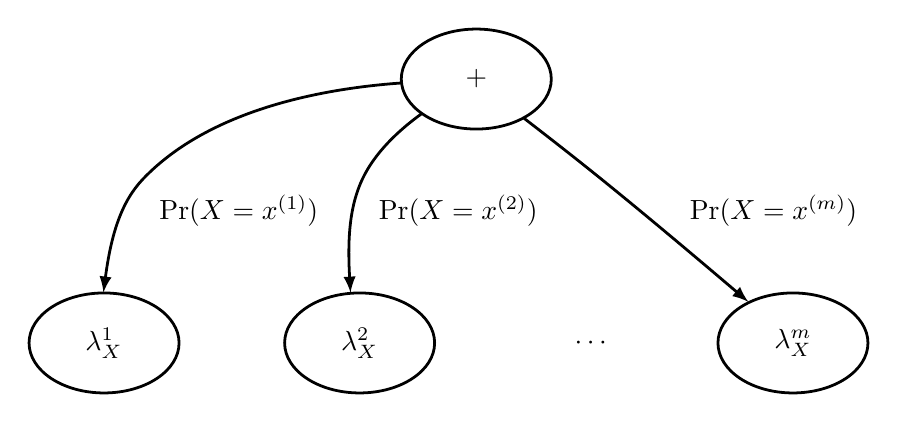
\begin{tikzpicture}[>=latex,line join=bevel,]
  \pgfsetlinewidth{1bp}
%%
\pgfsetcolor{black}
  % Edge: s -> l1
  \draw [->] (133.91bp,111.58bp) .. controls (106.62bp,109.65bp) and (65.194bp,102.36bp)  .. (41.0bp,77.0bp) .. controls (33.224bp,68.85bp) and (29.528bp,57.157bp)  .. (26.766bp,36.127bp);
  \definecolor{strokecol}{rgb}{0.0,0.0,0.0};
  \pgfsetstrokecolor{strokecol}
  \draw (75.5bp,65.5bp) node {$\Pr(X=x^{(1)})$};
  \draw (127.91bp,117.58bp) node {$$};
  \draw (20.766bp,42.127bp) node {$$};
  % Edge: s -> lm
  \draw [->] (178.21bp,98.855bp) .. controls (186.65bp,92.354bp) and (196.92bp,84.344bp)  .. (206.0bp,77.0bp) .. controls (221.22bp,64.695bp) and (238.03bp,50.572bp)  .. (258.97bp,32.769bp);
  \draw (268.0bp,65.5bp) node {$\Pr(X=x^{(m)})$};
  \draw (184.21bp,92.855bp) node {$$};
  \draw (252.97bp,38.769bp) node {$$};
  % Edge: s -> l2
  \draw [->] (141.35bp,100.55bp) .. controls (133.18bp,94.646bp) and (124.55bp,86.65bp)  .. (120.0bp,77.0bp) .. controls (115.54bp,67.536bp) and (114.53bp,56.199bp)  .. (115.73bp,36.079bp);
  \draw (154.5bp,65.5bp) node {$\Pr(X=x^{(2)})$};
  \draw (135.35bp,94.547bp) node {$$};
  \draw (109.73bp,42.079bp) node {$$};
  % Node: s
\begin{scope}
  \definecolor{strokecol}{rgb}{0.0,0.0,0.0};
  \pgfsetstrokecolor{strokecol}
  \draw (161.0bp,113.0bp) ellipse (27.0bp and 18.0bp);
  \draw (161.0bp,113.0bp) node {$+$};
\end{scope}
  % Node: lm
\begin{scope}
  \definecolor{strokecol}{rgb}{0.0,0.0,0.0};
  \pgfsetstrokecolor{strokecol}
  \draw (275.0bp,18.0bp) ellipse (27.0bp and 18.0bp);
  \draw (275.0bp,18.0bp) node {$\lambda_X^m$};
\end{scope}
  % Node: l2
\begin{scope}
  \definecolor{strokecol}{rgb}{0.0,0.0,0.0};
  \pgfsetstrokecolor{strokecol}
  \draw (119.0bp,18.0bp) ellipse (27.0bp and 18.0bp);
  \draw (119.0bp,18.0bp) node {$\lambda_X^2$};
\end{scope}
  % Node: cdots
\begin{scope}
  \definecolor{strokecol}{rgb}{0.0,0.0,0.0};
  \pgfsetstrokecolor{strokecol}
  \draw (203.0bp,18.0bp) node {$\cdots$};
\end{scope}
  % Node: l1
\begin{scope}
  \definecolor{strokecol}{rgb}{0.0,0.0,0.0};
  \pgfsetstrokecolor{strokecol}
  \draw (27.0bp,18.0bp) ellipse (27.0bp and 18.0bp);
  \draw (27.0bp,18.0bp) node {$\lambda_X^1$};
\end{scope}
%
\end{tikzpicture}


\end{center}

Note that this SPN is both complete, since the sum node's scope is $\{X\}$ and so are each of its
children's scope; and decomposable, since there are no product nodes.

%--------------------------------------------------------------------------------------------------

\newpage
\appendix

\newpage

\printbibliography[]

\end{document}
